El diseño de casos de pruebas para un proyecto de las características de \emph{Sitic}
es algo complicado, ya que necesitamos un escenario en el que interactúen todos los
elementos entre sí. Pero las pruebas son algo necesario si deseamos un software con una
calidad aceptable.

Todos los módulos que componen la aplicación han sido probados individualmente, como pueden
ser aquellos módulos encargados de la gestión de idiomas, generación de contenidos o categorización.

También se realizaron pruebas de integración, ya que había módulos, una vez probado en solitario,
debían realizar distintas acciones junto con otros módulos.

Otras pruebas que se realizaron fueron de generación, tanto yo como
personas ajenas al desarrollo de proyecto probaron el
mismo ofreciendo sus opiniones sobre aspectos que deberían ser modificados o
errores que aparecían a lo largo de la ejecución y en el resultado obtenido.

En definitiva, la organización de los casos de pruebas fue la siguiente:

\begin{enumerate}
    \item Tras finalizar la implementación de cada módulo, se realizaban pruebas unitarias sobre estos.
    \item A medida que distintos módulo que anteriormente probados individualmente, debían colaborar entre ellos, se
    llevaban a cabo pruebas de integración.
    \item Con las distintas versiones usables se realizaban pruebas de generación.
\end{enumerate}

\section{Pruebas unitarias}

Estas pruebas se realizaron junto a la fase de implementación, conforme se implementaban nuevos módulos para la aplicación,
se realizaban pruebas individuales sobre los mismos. De esta forma se buscaban todos los caminos posibles que podría dar cada
módulo, teniendo en cuenta aquellos que fueran más predispuesto a fallos.

De esta forma todas las sentencias se ejecutaban como mínimo una vez y los posibles fallos se encontraban de una forma más sencilla.
Por lo que también eran más fácil localizar donde estaba el problema y afrontar la solución.

% \subsection{Análisis del código con ylint.}
% 
% Una vez que se comprobaba el correcto funcionamiento del módulo implementado, se le pasaba el analizador de código pylint, con el
% fin de que el código siguiera un estándar uniforme y que estuviera exento de cualquier tipo de errores o signos de mala calidad.
% 
% Pylint proporciona una nota de 1 a 10 al código analizado. Se intentó que todos y cada uno de los módulos tuvieran al menos
% una nota mínima de 7. Finalmente se obtuvo una nota de 8.25 en todo el código conjunto de la aplicación.

\section{Pruebas de integración}

Conforme aparecían nuevos módulos, cuya implementación era necesaria y a su vez estos requerían el uso de otro módulos que
posteriormente habían sido probados individualmente, se realizaban pruebas de integración entre dichos módulos.

Conforme se avanzaba en el desarrollo, se realizaban pruebas de integración a mayor escala. No solo entre módulos
del mismo sistema, sino entre varios sistemas.

Una de las mejores formas que se pensaron para realizar este tipo de pruebas, fue desarrollar dos webs que usaran todos 
los elementos que se iban implementando.

En concreto se crearon las dos siguientes webs:

\begin{itemize}
    \item \textbf{Blog}: ejemplo de sitio web perfecto y sencillo, donde se pueden usar elementos como la paginación,
        taxonomías, comentarios, secciones y buscador. Se puede ver el resultado en la figura \ref{fig:blog-example}.
    \item \textbf{Documentación web}: otro ejemplo perfecto en el que se pueden ver somo se usan elementos como menús,
        internacionalización y buscador. Se puede ver el resultado en la figura \ref{fig:doc-example}.
\end{itemize}

\begin{figure}[htbp]
    \centering
    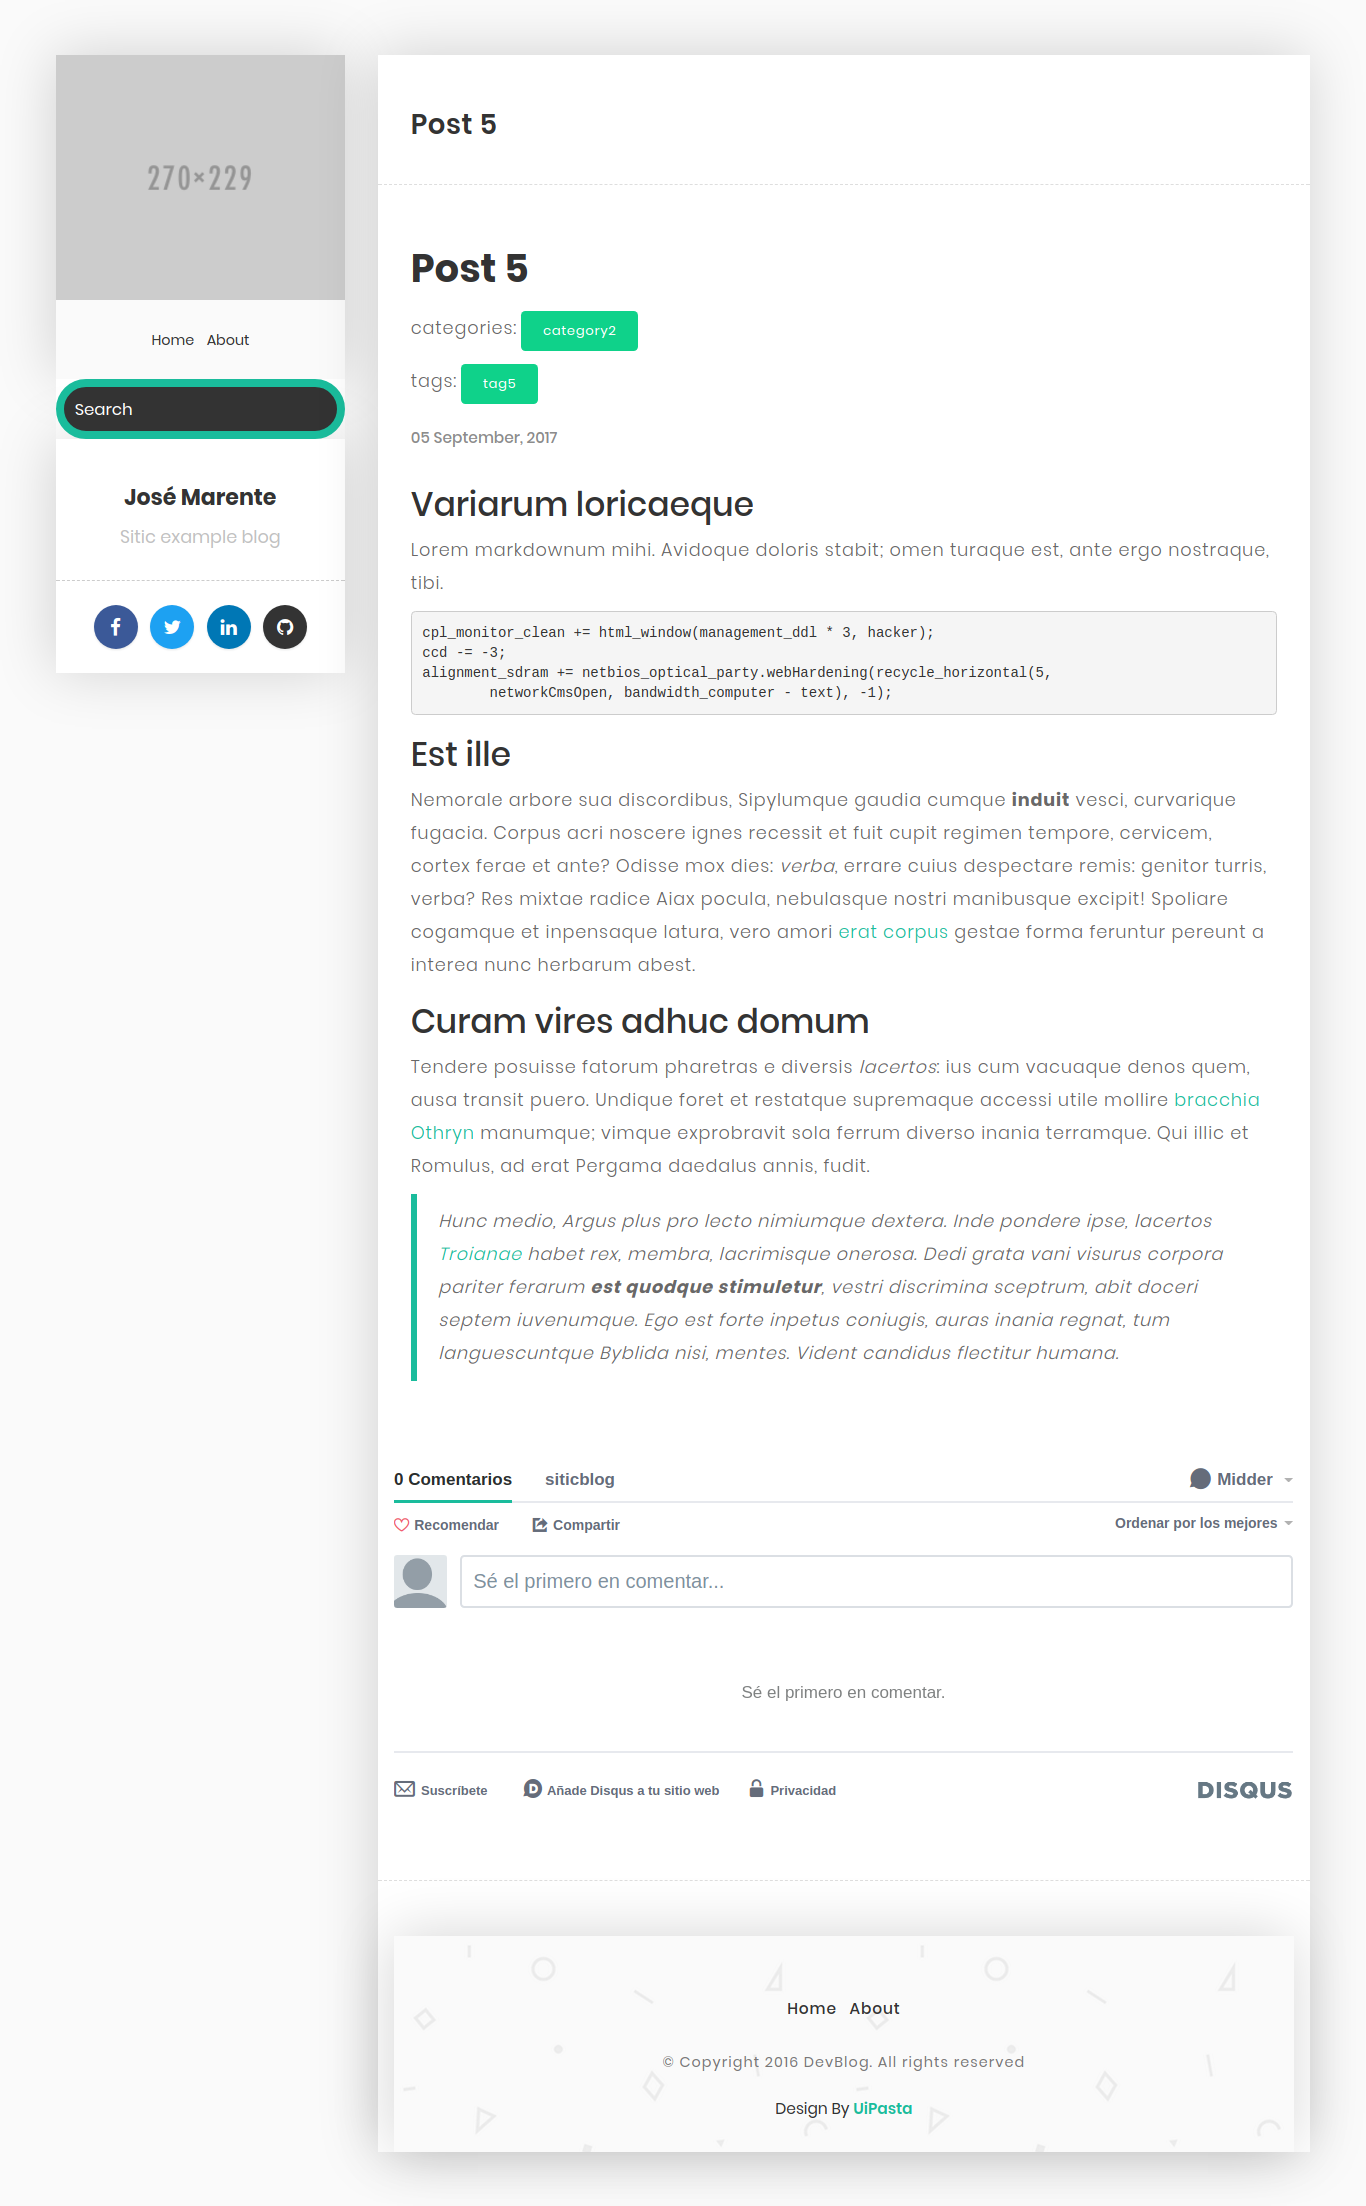
\includegraphics[width=1\textwidth]{7_pruebas/blog_example.png}
    \caption{Ejemplo de blog construido}
    \label{fig:blog-example}
\end{figure}

\begin{figure}[htbp]
    \centering
    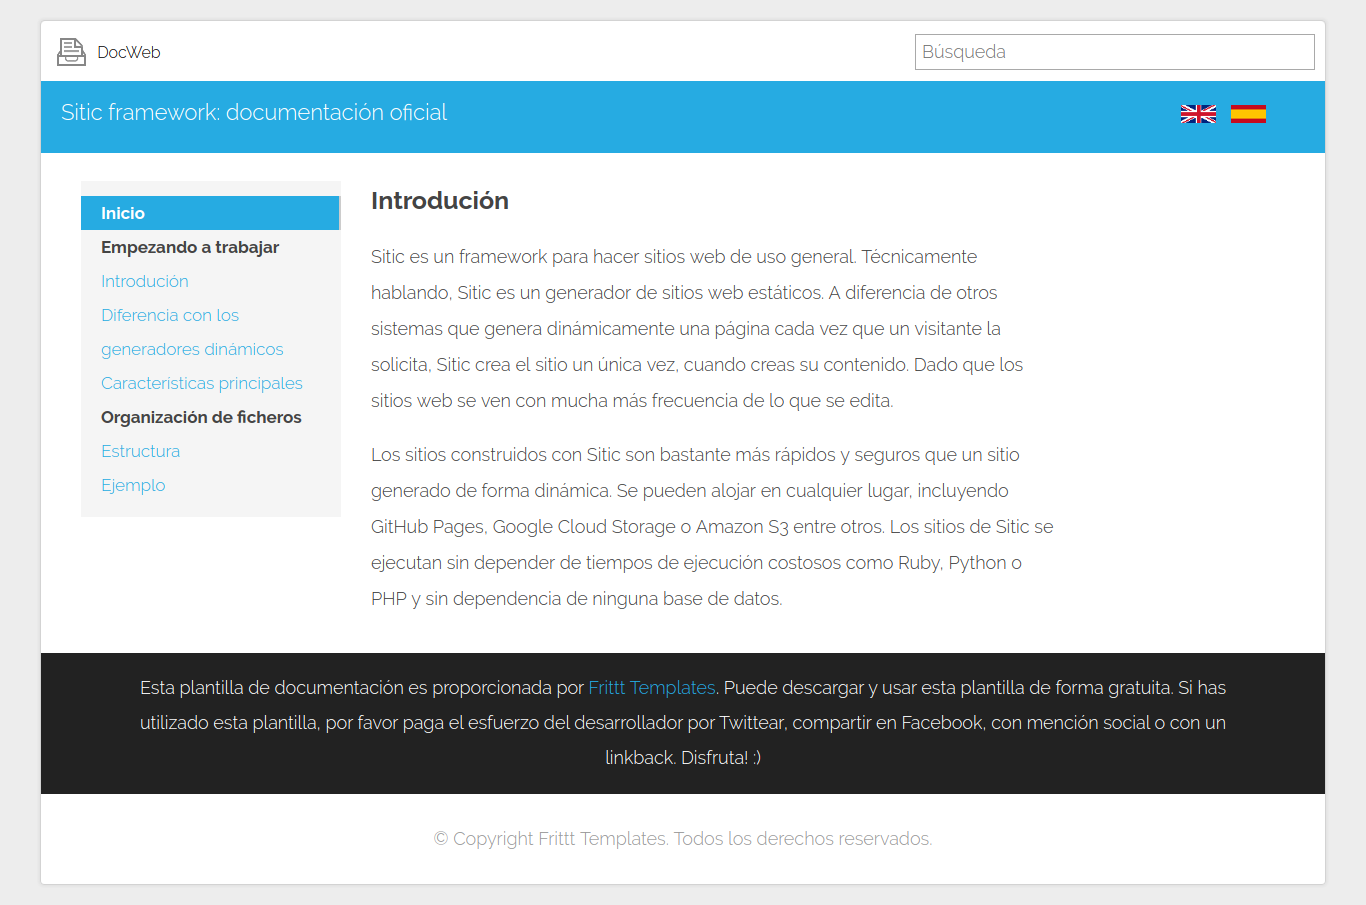
\includegraphics[width=1.1\textwidth]{7_pruebas/doc_example.png}
    \caption{Ejemplo de documentación web construido}
    \label{fig:doc-example}
\end{figure}

Ambos sitios están disponibles en el respositorio oficial del proyecto~\cite{repositorio}
bajo la carpeta \texttt{examples}.

Durante el desarrollo se descubrieron distintos errores y se mejoraron muchos aspectos de usabilidad del proyecto, 
como puede serel uso de las taxonomías o la usabilidad de la funcionalidad para la paginación de secciones.

\section{Pruebas de aceptación}

Conforme se avanzaba en el desarrollo del proyecto y se conseguían versiones estables del mismo, se
envíaban estas versiones, junto con el manual del proyecto, a un grupo de usuarios con los conocimientos
necesarios, capaces de interpretar los requerimientos especificados por los futuros usuarios de la herramienta.

El manual se iba actualizando con las nuevas funcionalidades que se iban añadiendo. De forma que
los usuarios pudieran identificar y probar correctamente todas las características de la herramienta.

Cada uno de estos usuarios devolvía un pequeño informe sobre la herramienta, en la que detallaban los distintos
problemas que se habían encontrado, errores que necesitaban ser corregidos y su opinión sobre
funcionalidades, indicando cuales podría ser ampliadas para que fueran más útiles o más sencillas de usar.

Con cada uno de estos informes, se trabajaba para mejorar la herramienta en versiones posteriores, dando
prioridad a aquellas que se consideraban más críticas.

Entre las principales quejas de los usuarios, se encontraban muchos aspectos referentes a los contenidos,
ya que algunos usuario consideraban que se debería permitir generar contenidos sin necesidad 
de generar ficheros en la carpeta de contenidos, por lo que se trabajó en una solución para corregirlo.

\section{Pruebas de generación}

Cada vez que estaban disponibles nuevas versiones estables de la herramienta, se pedían la ayuda a personas,
totalmente ajenas al desarrollo, que probaran las distintas versiones disponibles. De esta forma cada uno
de los colaboradores daba su opinión sobre  distintos aspectos como la usabilidad, dificultad, respuesta o eficiencia.
Tras recopilar la información que todos ellos proporcionaron, se procedía a realizar los ajustes
necesarios a los distintos parámetros requeridos.

Entre los distintos aspectos a probar que se le recomendaban a los
colaboradores que hicieran especial hincapié, son los siguiente:

\begin{itemize}
\item \textbf{Internacionalización}: definición de varios idiomas con contenidos divididos, así como pruebas de generar
los mismos contenidos sin ningún idioma configurado.
\item \textbf{Urls de ficheros}: definir distintas urls en los ficheros, comprobando que la generación se la ruta
se generaba de forma correcta, en función de la rutas definidas
\item \textbf{Paginación}: configurar distintos valores para la paginación de elementos por página, así como la desactivación
del mismo, comprobando que se generaban tantas páginas estáticas por sección/taxonomías como páginas debería de tener.
\item \textbf{Menús}: definición de menús con elementos estáticas y dinámicos.
\item \textbf{Categorización}: definir distintas taxonomías y mezclarlas entre los idiomas, comprobando finalmente que cada
contenido se había organizado de la forma correcta.
\end{itemize}
